\section{Linear Systems}
During this section, the following algorithms that we have implemented will be discussed:
\begin{itemize}
    \item LU Decomposition \algoref{alg:LU decomposition using Gaussian elimination} 
    \item Forward Decomposition \algoref{alg:Forward Substitution}
    \item Backward Decomposition \algoref{alg:Backward Substitution}
    \item LU Solver \algoref{alg:LU Solver}
    \item QR Factorization \algoref{alg:QR Factorization using Householder reflections}
    \item QR Solver \algoref{alg:QR Solver}
\end{itemize}

\subsection{LU Decomposition}
The (P)LU decomposition, developed in this package, factors a matrix into a product of three matrices PLU, P being the permutation matrix, L a lower triangular matrix and finally U an upper triangular matrix. This approach is usually used to solve linear problems; however, it may be applied in a variety of ways.

During the development of such method, some considerations have been taken into account; firstly, we put all the variables in the English language as well as a choosing a naming that will provide the future student some hints on what each variable is doing. 

Second, we established an auxiliary function that would execute the permutation, this function will have as an input the matrix $A$ and the number of the two rows to permute $i,j$; this option was made mostly for students to comprehend the stages prior to the use of notation; the notation for permuting was \lstinline|A[[i, j], :] = A[[j,i], :]|, so the development of a function that performs it will be easier for students to read.

Finally, we examine three main approaches that a student may take to develop lines 11–15 from \algoref{alg:LU decomposition using Gaussian elimination}, we will explore the various ways as well as the one built utilizing the well-known Scipy package in the next subsection, where we confirm that the choice of a for-loop is more efficient and easier to read.

This algorithm was primarly based upon Camilo's work \cite{bucheli2020}.

\subsubsection{Matrix reduction implmentation analysis}
We observed numerous methods a student may implement the LU Decomposition when designing it, which is why some discussion about whose implementation is superior should be addressed.

The multiple ways refers to the critical calculation of the reduction $ A'[row, col+1:n] \gets A'[row, col+1:n] - multiplier \cdot A'[col, col+1:n] $ , those ways could be enumerated as :

\begin{enumerate}
    \item By Submatrices Syntax
    \begin{lstlisting}[language=Python]
A[col + 1 :, col] = A[col + 1 :, col] / pivot
A[col + 1 :, col + 1 :] = A[col + 1 :, col + 1 :] - (A[col + 1 :, :][:, [col]] @ A[[col], :][:, col + 1 :])
    \end{lstlisting}

    \item By New Axis Syntax
    \begin{lstlisting}[language=Python]
A[col + 1 :, col] = A[col + 1 :, col] / pivot
A[col + 1 :, col + 1 :] = A[col + 1 :, col][:, np.newaxis] @ A[col, col + 1 :][np.newaxis, :]
    \end{lstlisting}

    \item By using the Outer Product
    \begin{lstlisting}[language=Python]
A[col + 1 :, col] = A[col + 1 :, col] / pivot
A[col + 1 :, col + 1 :] = np.outer(A[col + 1 :, col], A[col, col + 1 :])
    \end{lstlisting}

    \item Using a for loop
    \begin{lstlisting}[language=Python]
for row in range(col + 1, n):
    A[row, col] = A[row, col] / A[col, col]  # Calculate the multiplier and store in A for later use
    A[row, col + 1 :] = A[row, col + 1 :] - A[row, col] * A[col, col + 1 :]  # Update the remaining elements in the row using the multiplier
    \end{lstlisting} 
\end{enumerate}

To test these methods we will proceed by creating 100 random matrices for the sizes [500, 1000, 1500, 2000, 2500, 3000, 3500, 4000] and measure the length of time it takes for the algorithm to calculate the LU factorisation for each method. Note that all methods have exactly the same syntax before and after the options we have; therefore, we reduce possible noise.
\paragraph{Results}
The results of the mean of those 100 iterations for each size in seconds are as follows. 
\begin{table}[H]
    \centering
    \begin{tabular}{|l|l|l|l|l|l|}
    \hline
        \textbf{Matrix Size} & \textbf{Submatrices} & \textbf{New Axis} & \textbf{Outer Product} & \textbf{Loop} & \textbf{scipy} \\ \hline
        500 & 0.41335 & 0.169461 & 0.117083 & 0.465405 & 0.018257 \\ \hline
        1000 & 2.563606 & 1.522018 & 1.110119 & 2.176568 & 0.03057 \\ \hline
        1500 & 8.535015 & 5.212411 & 3.8087 & 5.579113 & 0.069611 \\ \hline
        2000 & 20.30588 & 12.333257 & 9.134406 & 10.942175 & 0.132066 \\ \hline
        2500 & 39.145535 & 23.998247 & 17.653031 & 19.098659 & 0.216267 \\ \hline
        3000 & 68.789119 & 41.919219 & 31.590708 & 29.468995 & 0.42402 \\ \hline
        3500 & 106.423081 & 64.700578 & 47.661064 & 42.445734 & 0.447992 \\ \hline
        4000 & 157.028937 & 96.519873 & 70.584879 & 58.448117 & 0.603978 \\ \hline
    \end{tabular}
    \caption{LU Methods Data in seconds}
\end{table}

on a visual plot:

\begin{figure}[H]
  \centering
    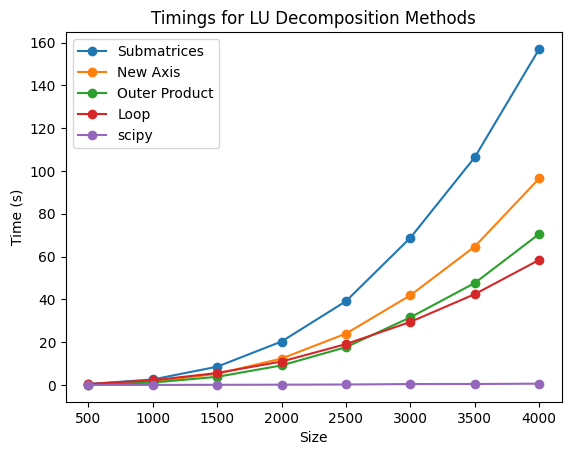
\includegraphics[scale=0.75]{Include/Images/Thesis/Analysis of Solutions/Linear Systems/LU Timings.png}
    \caption{LU Methods comparison}
    \label{fig:LU Methods comparison}
\end{figure}
\begin{figure}[H]
    \centering
    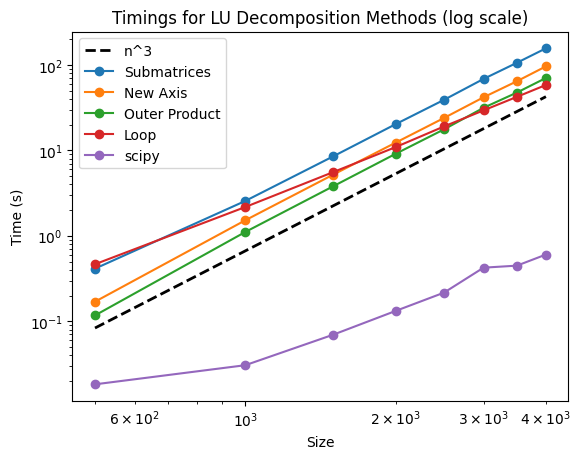
\includegraphics[scale=0.75]{Include/Images/Thesis/Analysis of Solutions/Linear Systems/LU Timings LOG.png}
    \caption{Log plot of LU methods}
    \label{fig:Log plot of LU methods}
\end{figure}

As we can observe from the tabular data and the plot, Scipy's method is by far the fastest, that is, due to the implementation using LAPACK's library, and the slowest is using the Submatrices syntax; surprisingly, the syntax using a for-loop improves over the other implementations as size increases, therefore even though this works for large sizes, using a for-loop that implements the reduction is the best choice overall the other methods (without accounting for Scipy's) 

For mere due diligence, we should also calculate the slopes using  linear regression.
\begin{table}[H]
    \centering
    \begin{tabular}{|l|l|l|l|l|l|}
    \hline
        \textbf{} & \textbf{Submatrices} & \textbf{New Axis} & \textbf{Outer Product} & \textbf{Loop} & \textbf{scipy} \\ \hline
        slope & 2.885234 & 3.043451 & 3.071779 & 2.334054 & 1.813654 \\ \hline
    \end{tabular}
    \caption{LU Data slopes of Linear Regression}
\end{table}
In this last table, we can see that although the submatrices syntax was the slowest in the previous plots, is better than using the New Axis syntax, it must be noted that this will only be seen when the size of the matrix is humongous, and barely reachable in a sort span of time. 

\subsubsection{Examples}
	\paragraph{Example 1}{
\begin{lstlisting}[language=Python]
from BNumMet.LinearSystems import lu
A = np.array([[10, -7, 0], [-3, 2, 6], [5, -1, 5]])
P, L, U = lu(A)
display(P, L, U)

>> P = array([ [1., 0., 0.],
               [0., 0., 1.],
               [0., 1., 0.]])
>> L = array([ [ 1.  ,  0.  ,  0.  ],
               [ 0.5 ,  1.  ,  0.  ],
               [-0.3 , -0.04,  1.  ]])
>> U = array([ [10. , -7. ,  0. ],
               [ 0. ,  2.5,  5. ],
               [ 0. ,  0. ,  6.2]])
           
\end{lstlisting}
}


\subsection{Forward and Backward Substitution}
Undoubtedly, one of the key steps in solving a linear system is substitution, where we find the actual solutions to our system, that is why there exists two main numerical methods that are use, which are Forward and Backward substitution. These methods take a triangular matrix (lower and upper, respectively) and make the necessary substitutions.

The first approach, forward substitution, substitutes the first row and then moves "forward" in the next variables using the already computed values. Backward substitution is analogous, but instead of starting with the first variable, it starts with the last (since this method takes an upper triangular matrix) and moves backwards until it has reached the first variable.

The reason of implementing this method is that independently of the decomposition, these methods are also taught in universities and is a good exercise for any student to try.

The algorithms were based upon Fernando Terán de Vergara's course notes for the Master in Applied \& Computational Mathematics \cite{Vergara}.
\subsubsection{Examples}
\textbf{Forward Substitution}
	\paragraph{Example 1}{
\begin{lstlisting}[language=Python]
from BNumMet.LinearSystems import lu, forward_substitution
A = np.array([[10, -7, 0], [-3, 2, 6], [5, -1, 5]])
b = np.array([7, 4, 6])
P, L, U = lu(A)
solution_aux = forward_substitution(L, P @ b)
display(solution_aux)

>> solution_aux = array([7. , 2.5, 6.2])
\end{lstlisting}
}

 \textbf{Backward Substitution}
	\paragraph{Example 1}{
\begin{lstlisting}[language=Python]
from BNumMet.LinearSystems import lu, forward_substitution, backward_substitution
A = np.array([[10, -7, 0], [-3, 2, 6], [5, -1, 5]])
b = np.array([7, 4, 6])
P, L, U = lu(A)
solution_aux = forward_substitution(L, P @ b)
solution = backward_substitution(U, solution_aux)
display(solution)

>> solution = array([ 0., -1.,  1.])
\end{lstlisting}
}
\subsection{QR Decomposition}
Alongside the LU decomposition, there exists another decomposition known as the QR Decomposition, similarly to the LU decomposition, the concept behind QR is decompose a matrix into a product of two, in this case, it will be a product of an orthogonal matrix (Q) and an upper triangular (R). We have implemented this technique using Householder reflectors which is the fundamental method that is taught in universities when QR is being introduced.

The reason of implementing these method as a standalone is to give an additional feature to BNumMet and also to the students. Though a QR solver is used to solve the Least Squares problem, these method as an autonomous is not used, only an optimized variant for the solver which takes into consideration the independent terms.

The algorithm was based upon Fernando Terán de Vergara's course notes for the Master in Applied \& Computational Mathematics \cite{Vergara}.
\subsubsection{Examples}
\paragraph{Example 1}{
\begin{lstlisting}[language=Python]
from BNumMet.LinearSystems import qr_factorization
A = np.array([[10, -7, 0], [-3, 2, 6], [5, -1, 5]])
Q, R = qr_factorization(A)
display(Q,R)

>> Q  = 
    array([[-0.86386843,  0.42560398,  0.26943013],
           [ 0.25916053, -0.08312578,  0.96225045],
           [-0.43193421, -0.90108343,  0.03849002]])
>> R = 
    array([[-11.5758369 ,   6.99733425,  -0.6047079 ],
           [  0.        ,  -2.24439601,  -5.00417184],
           [  0.        ,   0.        ,   5.96595278]])
>> Q@R = 
    array([[ 1.00000000e+01, -7.00000000e+00, -4.67352964e-16],
           [-3.00000000e+00,  2.00000000e+00,  6.00000000e+00],
           [ 5.00000000e+00, -1.00000000e+00,  5.00000000e+00]])
\end{lstlisting}
}

\subsection{LU Solver}
We implemented the function that solves a linear system $Ax=b$ using the LU factorization and forward and backward substitution as part of the Linear Systems Package. The reason for implementing these is to add extra features to BNumMet as well as give the student a written version of the solver, as it is trivial to implement once you have the aforementioned methods. Apart from appropriately commenting the code, no other considerations have been made.
\subsubsection{Examples}
	\paragraph{Example 1}{
\begin{lstlisting}[language=Python]
from BNumMet.LinearSystems import lu_solve
A = np.array([[10, -7, 0], [-3, 2, 6], [5, -1, 5]])
b = np.array([7, 4, 6])
solution = lu_solve(A, b)
display(solution)

>> solution = array([ 0., -1.,  1.])
\end{lstlisting}
}

\subsection{QR Solver}
Similarly to the LU Solver, we have added a functionality that will be critical on solving the Least Squares Problem, that is the QR solver. The reason for the QR solver, aside from being used in the Least Squares Problem to avoid the ill-conditioning of solving the Least Squares Problem using the well-known formula of $A^T A x= A^T b$, is that we find it curious because it implements an optimized version of QR taking into account the fact that we are solving a Linear System, in this optimized version, the algorithm does not compute the Q matrix but rather it applies it to the independent terms and then uses the backward substitution on R (which is computed).

Not only does this method will provide student with another approach on solving linear systems or the Least Squares Problem, but it also grants the underlying procedure of the well-known Matlab Backslash.

The algorithm is based upon Cleve's and Fernando Terán's work \cite{Vergara,doi:10.1137/1.9780898717952}
\subsubsection{Examples}
\paragraph{Example 1}{
\begin{lstlisting}[language=Python]
from BNumMet.LinearSystems import qr_solve
A = np.array([[10, -7, 0], [-3, 2, 6], [5, -1, 5]])
b = np.array([7, 4, 6])
solution = qr_solve(A, b)
display(solution)

>> solution = 
        array([-3.83634647e-16, -1.00000000e+00,  1.00000000e+00])
\end{lstlisting}
}


